\section{Inference-Time Defences Cut False Acceptance by Rejecting Passing Plans}\label{sec:defences}

\begin{figure*}[tbp]
\centering
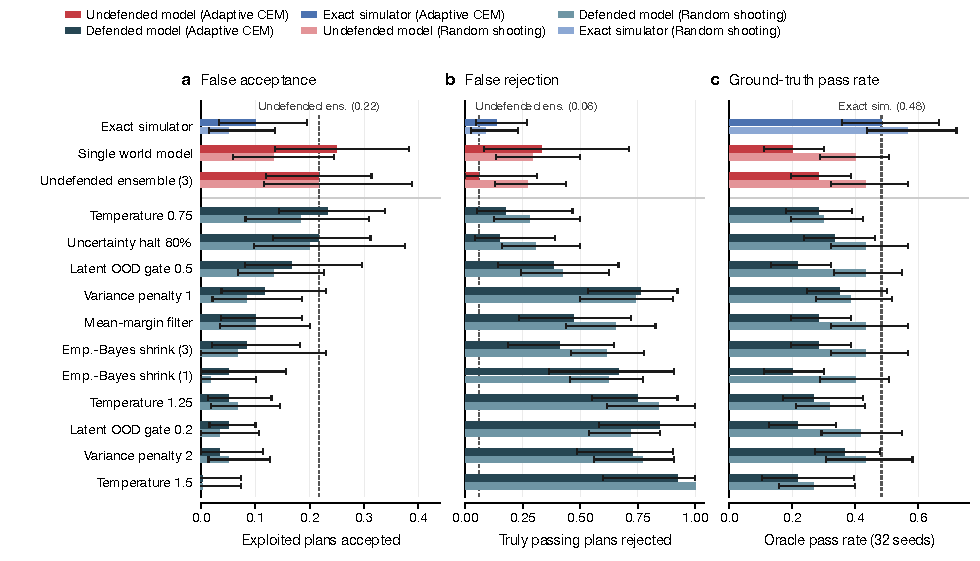
\includegraphics[width=\textwidth]{figures/fig_defences.pdf}
\caption{\textbf{Inference-time world-model defences trade reduced false acceptance directly for elevated false rejection without recovering ground-truth discovery.} Evaluation across \DefInstances{} instances (\DefFamilies{} cities) at $B ={}$\Bp{3} under adaptive CEM (saturated bars) and random shooting (light-tinted bars), showing \textbf{a}, false acceptance, \textbf{b}, false rejection of truly passing selections, and \textbf{c}, \OracleSeeds-seed ground-truth oracle pass rate (error bars denote \CILevel{} per cent cluster-bootstrap intervals; vertical dashed lines mark the undefended ensemble in \textbf{a}, \textbf{b} and the exact-simulator reference in \textbf{c}). Top rows show the exact-simulator reference (steel blue) alongside the single primary model and undefended \DefMembers-member seed ensemble (crimson); lower rows show regularisers spanning variance penalties, mean-margin filtering, empirical-Bayes shrinkage, sampling temperatures, uncertainty halts, and cross-fitted latent OOD gates (deep petrol; Appendix~\ref{app:defences}).}
\label{fig:defences}
\end{figure*}

When retraining is infeasible, model-based pipelines rely on inference-time regularisation. Across \DefInstances{} instances (\DefFamilies{} cities) at $B ={}$\Bp{3}, we test \DefTestedN{} canonical defences across five families on a \DefMembers-member seed ensemble of budget-matched \SizeM{} models (Appendices~\ref{app:searches} and~\ref{app:defences}). These span sampling temperatures \citep{ha2018worldmodels}, empirical-Bayes pass-share shrinkage \citep{smith2006optimizer}, MOPO-style disagreement penalties \citep{yu2020mopo} (including a zero-weight positive-margin control), MOReL-style uncertainty halts \citep{kidambi2020morel}, and a cross-fitted logistic OOD detector.

Two results stand out (Figure~\ref{fig:defences}). First, naive ensembling alone (\DefKSearchEns{} search and \DefKVerdictEns{} verdict rollouts across \DefMembers{} members vs.\ \DefKSearch{} and \DefKVerdict{} for one model) does not reliably curb exploitation. Under random shooting, the undefended \DefMembers-member ensemble incurs \DefEnsHack{} \ci{\DefEnsHackCI} false acceptance versus \DefMemberHack{} \ci{\DefMemberHackCI} for its primary member (false rejection \DefEnsFalseRej{} vs.\ \DefMemberFalseRej{}), as averaging correlated biases sharpens confidence on shared errors. Under adaptive CEM, it slightly trims false acceptance (\DefAdEnsHack{} \ci{\DefAdEnsHackCI} vs.\ \DefAdMemberHack{} \ci{\DefAdMemberHackCI}) and lowers false rejection from \DefAdMemberFalseRej{} to \DefAdEnsFalseRej{}.

Second, every post-hoc regulariser that meaningfully cuts false acceptance pays for it by discarding many truly passing plans. Across all \DefEnsTestedN{} ensemble defences under shooting, the \DefSigN{} configurations whose false-acceptance reductions exclude zero falsely reject \DefSigFalseRejMin{}--\DefSigFalseRejMax{} of truly passing selections (vs.\ \DefEnsFalseRej{} undefended). Most of MOPO's reduction already occurs at penalty weight zero (false acceptance \DefPenZeroHack{}, false rejection \DefPenZeroFalseRej{}) via threshold tightening rather than variance penalisation. Meanwhile, the OOD detector drops from \DetAucMin{}--\DetAucMax{} ROC AUC on logged plans to \DetSelAuc{} \ci{\DetSelAucCI} on search-selected plans. Adaptive CEM faces the same trade-off (Figure~\ref{fig:defences}a--c), with the \DefAdSigN{} effective defences rejecting \DefAdSigFalseRejMin{}--\DefAdSigFalseRejMax{} of passing plans (vs.\ \DefAdEnsFalseRej{} undefended) and none raising ground-truth pass rates. Screening the top choice once on the true simulator removes false acceptance at zero rejection cost, leaving ground-truth discovery during search as the core bottleneck.
